\documentclass[a4paper, 12pt]{article} % Uses article class in A4 format

%----------------------------------------------------------------------------------------
%	FORMATTING
%----------------------------------------------------------------------------------------

\addtolength{\hoffset}{-2.25cm}
\addtolength{\textwidth}{4.5cm}
\addtolength{\voffset}{-3.25cm}
\addtolength{\textheight}{5cm}
\setlength{\parskip}{0pt}
\setlength{\parindent}{0in}

%----------------------------------------------------------------------------------------
%	PACKAGES AND OTHER DOCUMENT CONFIGURATIONS
%----------------------------------------------------------------------------------------

\usepackage{charter} % Use the Charter font
\usepackage[utf8]{inputenc} % Use UTF-8 encoding
\usepackage{microtype} % Slightly tweak font spacing for aesthetics

\usepackage[english]{babel} % Language hyphenation and typographical rules

\usepackage{amsthm, amsmath, amssymb} % Mathematical typesetting
\usepackage{float} % Improved interface for floating objects
\usepackage[final, colorlinks = true, 
            linkcolor = black, 
            citecolor = black]{hyperref} % For hyperlinks in the PDF
\usepackage{graphicx, multicol} % Enhanced support for graphics
\usepackage{color}
\usepackage{xcolor} % Driver-independent color extensions
\usepackage{marvosym, wasysym} % More symbols
\usepackage{rotating} % Rotation tools
\usepackage{censor} % Facilities for controlling restricted text
\usepackage{listings} % Environment for non-formatted code
\usepackage{algorithm}
\usepackage{algpseudocode} % Environment for specifying algorithms in a natural way
\renewcommand{\algorithmicrequire}{\textbf{Input:}}
\renewcommand{\algorithmicensure}{\textbf{Output:}}
\renewcommand{\algorithmicreturn}{\textbf{Return:}}
\usepackage{booktabs} % Enhances quality of tables

\usepackage{cases}
\usepackage{bookmark}

\usepackage{tikz-qtree} % Easy tree drawing tool
\tikzset{every tree node/.style={align=center,anchor=north},
         level distance=2cm} % Configuration for q-trees

\usepackage[backend=biber,style=numeric,
            sorting=nyt]{biblatex} % Complete reimplementation of bibliographic facilities

\usepackage{csquotes} % Context sensitive quotation facilities

\usepackage[yyyymmdd]{datetime} % Uses YEAR-MONTH-DAY format for dates
\renewcommand{\dateseparator}{-} % Sets dateseparator to '-'

\usepackage{fancyhdr} % Headers and footers
\pagestyle{fancy} % All pages have headers and footers
\fancyhead{}\renewcommand{\headrulewidth}{0pt} % Blank out the default header
\fancyfoot[L]{} % Custom footer text
\fancyfoot[C]{} % Custom footer text
\fancyfoot[R]{\thepage} % Custom footer text

\newcommand{\note}[1]{\marginpar{\scriptsize \textcolor{red}{#1}}} % Enables comments in red on margin


\definecolor{codegreen}{rgb}{0,0.6,0}
\definecolor{codegray}{rgb}{0.5,0.5,0.5}
\definecolor{codemauve}{rgb}{0.58,0,0.82}

\lstset{ %
	language=python,                % choose the language of the code
	basicstyle=\footnotesize\ttfamily,       % the size of the fonts that are used for the code
	numbers=left,                   % where to put the line-numbers
	numberstyle=\tiny\color{codegray},      % the size of the fonts that are used for the line-numbers
	stepnumber=1,                   % the step between two line-numbers. If it is 1 each line will be numbered
	numbersep=5pt,                  % how far the line-numbers are from the code
	backgroundcolor=\color{white},  % choose the background color. You must add \usepackage{color}
	showspaces=false,               % show spaces adding particular underscores
	showstringspaces=false,         % underline spaces within strings
	showtabs=false,                 % show tabs within strings adding particular underscores
	frame=single,                   % adds a frame around the code
	tabsize=4,                      % sets default tabsize to 4 spaces  
	captionpos=b,                   % sets the caption-position to bottom
	breaklines=true,                % sets automatic line breaking
	breakatwhitespace=false,        % sets if automatic breaks should only happen at whitespace
	escapeinside={\%*}{*)},
	commentstyle=\color{codegreen},
	keywordstyle=\bfseries\color{magenta},
	stringstyle=\color{red},
	identifierstyle=\color{codemauve},
	keepspaces=true
}

%----------------------------------------------------------------------------------------

\begin{document}

%----------------------------------------------------------------------------------------
%	TITLE SECTION
%----------------------------------------------------------------------------------------

\fancyhead[C]{}
\hrule \medskip % Upper rule
\begin{minipage}{0.295\textwidth} % Left side of title section
	\raggedright
	DATA130045\\ % Your course code
	\footnotesize % Authors text size
	\hfill\\
	Graph Data Management and Mining\\ % Your course name
\end{minipage}
\begin{minipage}{0.4\textwidth} % Center of title section
	\centering
	\large % Title text size
	\textbf{Final Project}\\ % Assignment title and number
	\normalsize % Subtitle text size
	\textbf{SimRank Enhanced by Semantic}\\ % Assignment subtitle
\end{minipage}
\begin{minipage}{0.295\textwidth} % Right side of title section
	\raggedleft
	Tim Walker\\ % Your name
	\footnotesize % Email text size
	\hfill\\
	\today\\ % Date
\end{minipage}
\medskip\hrule % Lower rule
\bigskip

%----------------------------------------------------------------------------------------
%	ARTICLE CONTENTS
%----------------------------------------------------------------------------------------

\section*{\textbf{Abstract}}
    
    SimRank is a widely used and popular measurement to evaluate the similarity among the vertices. However, with more and more graphs involves some of the labels that contain semantic message, the original SimRank might fail to deal with some of the queries. In our final report we will present comprehensive explanation about our idea and some of the experiments done by us.


\bigskip

%------------------------------------------------

\section{Introduction}
    
    Estimating node similarity with SimRank is a well-established technique that we have several high efficient ways to calculate the approximate SimRank (or accurate one). However, the traditional SimRank only consider the structure of the graph itself, but neglect the labels in the informative networks, which could be a great loss of information on the query of such networks. Therefore, some papers have already done some research on this field, presented different solutions for the semantic-enhanced SimRank computation.
    
    As we know most of the SimRank-based top-k queries on large graph use the randomwalk-based method, and the variants of the method have been proved efficient and could handle most of the cases. The READS method is a pretty efficient method to calculate the SimRank on graphs without label, it is also used in LSimRank to boost the calculation of semantic-enhanced SimRank. However, no matter the SemSim or LSimRank, the way they transfer information during random walk is an inseparable opperation. For instance, the core equation of SemSim is 
    
    \begin{equation}
        \frac{\operatorname{sem}(u, v) \cdot c}{N_{u, v}} \sum_{i}^{|I(u)||I(v)|} \sum_{j} \operatorname{sim}\left(I_{i}(u), I_{j}(v)\right) \cdot W\left(I_{i}(u), u\right) \cdot W\left(I_{j}(v), v\right)
    \end{equation}
    
    The part $\operatorname{sem}(u, v)$ increase the difficulty of randomwalk, which, in the graph similarity query problem neglect the labels, they only need to store the $Next_i$ index, which is $O(n)$ storage complexity for each round of simulation. But for SemSim or LSimRank, if they adopt the framework of READS method (or other approximation methods), the path of each randomwalk must be stored for the similarity computation. Which not only increase the storage complexity, but also increase the query time as they need to backtrace the path in each round of offline simulation.
    
    To handle the above situation, as the weight of the edge in equation (1) could be added into READS with simple modify of the origin algorithm, we want to make use of the weight of edges in the graph to transfer the semantic information. Therefore, we think the paper of Semantic Proximity Search might help us with forming the proper edge weight.

\bigskip

\section{Offline Phase}
    \subsection{Metagraph Matching}
    
    We hinge on the novel insight that different semantic classes can often construct structures in common, namely metagraph. Based on the previous method called GRAMI algorithm, the metagraph patterns could be generated automatically according to frequent pattern mining.
    
    Then we propose a supervised approach that identifies the characteristic metagraph, in practice, we learn a weight for each metagraph to quantify how well it can stand the specific class.
    
    \begin{figure}[H]
        \centering
        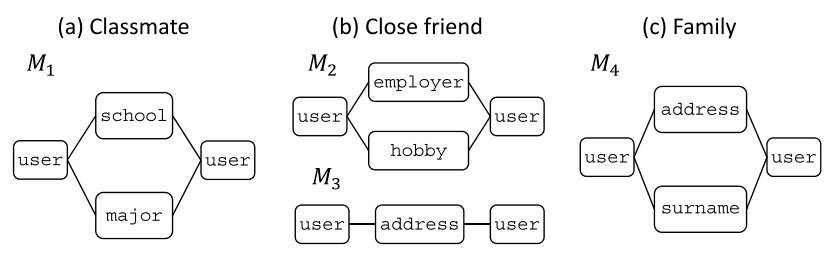
\includegraphics[width=0.5\textwidth]{img/metagraph.jpg}
        \caption{Possible Toy Metagraphs for some Classes}
    \end{figure}
    
    After implementing this, it comes to metagraph matching. While it is proved that computing the instances of a metagraph is highly costly, which is equivalent to solving a NP-hard subgraph matching problem, we shall work on another clever way that re-uses "symmetic" characteristic. As a result, we can avoid redundancy and substantially improve the efficiency of metagraph matching.
    
    In order to know whether two nodes share a characteristic metagraph pattern for the specific type of proximity, it is crucial to identify subgraph on the whole object graph that match instances of any metagraph.
    
    Before leading to our weight formula, here're some notations denotes the number of instances of each metagraph that matches between nodes.
    
    \begin{equation}
        \mathbf{m}_{x y}[i] & \triangleq \mid\left \{S \in \mathcal{I}\left(M_{i}\right) \mid \text { ContainsSym }(S, x, y)\right \} \mid
    \end{equation}
    
    \begin{equation}
        \mathbf{m}_{x}[i] & \triangleq \mid\left\{S \in \mathcal{I}\left(M_{i}\right) \mid \exists_{y \neq x} \text { ContainsSym }(S, x, y)\right\} \mid
    \end{equation}

    \subsection{TF-IDF-like Formula}
    
    As for the original Metagraph Matching, we could define different kinds of relations, and distinguished by different pattern and pattern weight, we could easily compute the similarity between nodes. But in many cases, we need to find the similarity between nodes without specific relation, which means, the relation itself also could be important or not. Therefore we make use of the TF-IDF method in LSA and present the importance of each in-neighbor of node $x$ in the following way:
    
    \begin{equation}
        \sum\limits_{\omega_{i}}\frac{m_{x y}^{T} \omega_i}{m_{x}^{T} \omega_i+m_{y}^{T} \omega_i} \log \frac{|E| e^{T} \omega_{i}}{\sum m_{x y}^{T} \omega_{i}}
    \end{equation}
    
    Where $m_{x}$ and $m_{xy}$ means metagraph vector for node $x$ and node pair $x$, $y$, respectively. $w$ indicates characteristic weight vector.
    
    After normalization, we could sample each in-neighbor of node $x$ with specific probability to specify its importance.
    
    \subsection{READS Offline Indexing}
    
    In the problem concerning simple SimRank query without label, the READS framework provides a way to construct efficiency index for online query, and it only require small amount of storage. The basic idea is, in the original randomwalk method, we have
    
    \begin{equation}
        s(u, v)=\sum_{i=1}^{t} \operatorname{Pr}\left(f\left(\pi_{u}, \pi_{v}\right)=i\right) \times c^{i}
    \end{equation}
    
    Thus, to calculate the approximation of SimRank, we need to store the length of two randomwalk before their first meet. To improve it, READS use different way to sample the in-neighbor of a node, which could be present as follow
    
    \begin{equation}
        \begin{array}{|l|l|}
            \hline \mathbf{a} & \operatorname{Pr}\left(u_{1}=v\right)=\frac{1}{\left|\operatorname{In}\left(u_{0}\right)\right|} \text { for } v \in \operatorname{In}\left(u_{0}\right) \\
            \hline \mathbf{b} & \operatorname{Pr}\left(u_{i+1}=v\right)=\frac{\sqrt{c}}{\left|\operatorname{In}\left(u_{i}\right)\right|} \text { for } v \in \operatorname{In}\left(u_{i}\right), 0<i<t \\
        \hline
        \end{array}
    \end{equation}
    
    With this kind of sampling technique, the randomwalk might stop at certain step, which means it contains the probability that two path will not meet within the step limitation. Therefore, we have the following equation
    
    \begin{equation}
        s(u, v)=\sum_{i=1}^{t} \operatorname{Pr}^{S A}\left(f\left(\pi_{u}, \pi_{v}\right)=i\right) \times c
    \end{equation}
    
    From which we could see that no matter how many steps does the simulation takes for two reverse randomwalk to meet, they all have the same amount of contribution to the SimRank. That is to say, to calculate the approximation of SimRank of two nodes $u, v$, all we need to do is simply counting the number of time that the two reverse randomwalk starting from $u, v$ meet each other in the total $r$ rounds, and each of them has the contribution of $c / r$. We could present this outcome with the following equation
    
    \begin{equation}
        \begin{split}
            s(u, v) &= \sum_{i=1}^{t} \operatorname{Pr}^{S A}\left(f\left(\pi_{u}, \pi_{v}\right)=i\right) \times c \\
            & \approx \widetilde{\operatorname{Pr}}^{S A}\left(f\left(\pi_{u}, \pi_{v}\right) \neq \infty\right) \\
            &= \left|\left\{j \leq r \mid f\left(\pi_{u}^{j}, \pi_{v}^{j}\right) \neq \infty\right\}\right| / r \\
        \end{split}
    \end{equation}
    
    With the above outcome, we could deploy the corresponding simulation. In each round of simulation, we start from leaf nodes, i.e. all the nodes on the graph, and deploy reverse randomwalk from all the leaf nodes with the above rules. If two randonwalk meet each other, they will simply merge to each other and continue doing reverse randomwalk as one branch instead of two separate branches. A branch of reverse randomwalk will stop once it has the length of $t$, i.e. the limitation of maximum randomwalk steps, or it stops as the above rules. Then we will attain a forest, which to check whether two randomwalks meet each other, we just need to check if the two nodes on the same tree, and we could form a index which is handy and easy for query. Here is an example
    
    \begin{figure}[H]
        \centering
        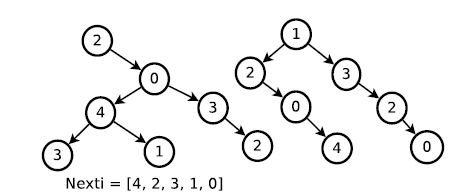
\includegraphics[width=0.4\textwidth]{img/READS forest.png}
        \caption{READS Example}
        \label{fig:READS}
    \end{figure}
    
    The $i^{th}$ element of $Nexti$ represents the right sibling of leaf node $i$, if $i$ is the rightmost leaf node in the tree, then $Nexti[i]$ represents the leftmost node in the tree. In this case, we have node 4's right sibling is 0, so $Nexti[4] = 0$. Thus, each round of simulation only takes $O(n)$ of storage, with $r$ rounds of simulation we only need $O(rn)$ of storage (The effect of $c$ will make all the tree really short, thus we could take the height of tree as a small constant).
    
    \subsection{REAEDS with Weight on the Edges}
    
    To make use of the information of edge weight, we just need to adjust the sampling rule in (4) in the following way
    
    \begin{equation}
        \begin{array}{|l|l|}
            \hline \mathbf{a'} & \operatorname{Pr}\left(u_{1}=v\right)=\frac{W(v, u_0)}{W(u_0)} \text { for } v \in \operatorname{In}\left(u_{0}\right) \\
            \hline \mathbf{b'} & \operatorname{Pr}\left(u_{i + 1}=v\right)=\frac{W(v, u_i)}{W(u_i)} \text { for } v \in \operatorname{In}\left(u_{i}\right), 0<i<t \\
        \hline
        \end{array}
    \end{equation}
    
    Where $W(u, v)$ stands for the weight of edge $(u, v)$, and $W(u) = \sum\limits_{v \in \operatorname{In}\left(u\right)} W(v, u)$
    
\bigskip

%------------------------------------------------

\section{Online Phase}

    The Online Phase is simple for READS framework. To calculate one-to-all query, using the outcome of the former chapter, we have the following algorithm
    
    \begin{algorithm}[H]
        \caption{One-to-all Query}
        \begin{algorithmic}[1]
            \Require Next, u
            \Ensure $s_1(u, *)$
            \For{i = 1:r}
                \State $v \gets Next_i[u]$
                \While{$v \neq u$}
                    \State $s_1(u, v) += c/r$
                    \State $v \gets Next_i[v]$
                \EndWhile
            \EndFor
            \State $s_1(u, u) \gets 1$
            \Return $s_1(u, *)$
        \end{algorithmic}
    \end{algorithm}

\bigskip

%------------------------------------------------

\section{Experiments}

    We implemented our ideas above in order to demonstrate two goals. First, our implementation can return query results as quickly as possible. Second, the output can be validated to show that sematic information truly improves the accuracy.

    \subsection{\textbf{Dataset}}
    
    To test our algorithm's efficiency, we use the following three datasets, one is the famous LinkedIn dataset with sematic labels, one is Facebook, and the other is self-constructed social network, which is taken from the real classmates around us.
    
    \begin{center}
        \begin{tabular}{c|ccccc}
        \hline & \#Nodes & \#Edges & \#Types & \#Metagraphs & \#Queries \\
        \hline
        LinkedIn & 65925 & 220812 & 4 & 164 & 172 \\
        Facebook & 5025 & 100356 & 10 & 954 & 904 \\
        FudanDS & 67 & 712 & 3 & 10 & 10 \\
        \hline
        \end{tabular}
    \end{center}

    We conducted extensive expriments on the real-world datasets LinkedIn, Facebook and FudanDS. All datasets contain features of various types. In particular, LinkedIn included user, employer, location and college. Facebook included user, major, degree, school, hometown, surname, location, employer, work-loaction, work-project and others. FudanDS included research direction, dormitory and social cycle.
    
    \begin{figure}[H]
        \centering
        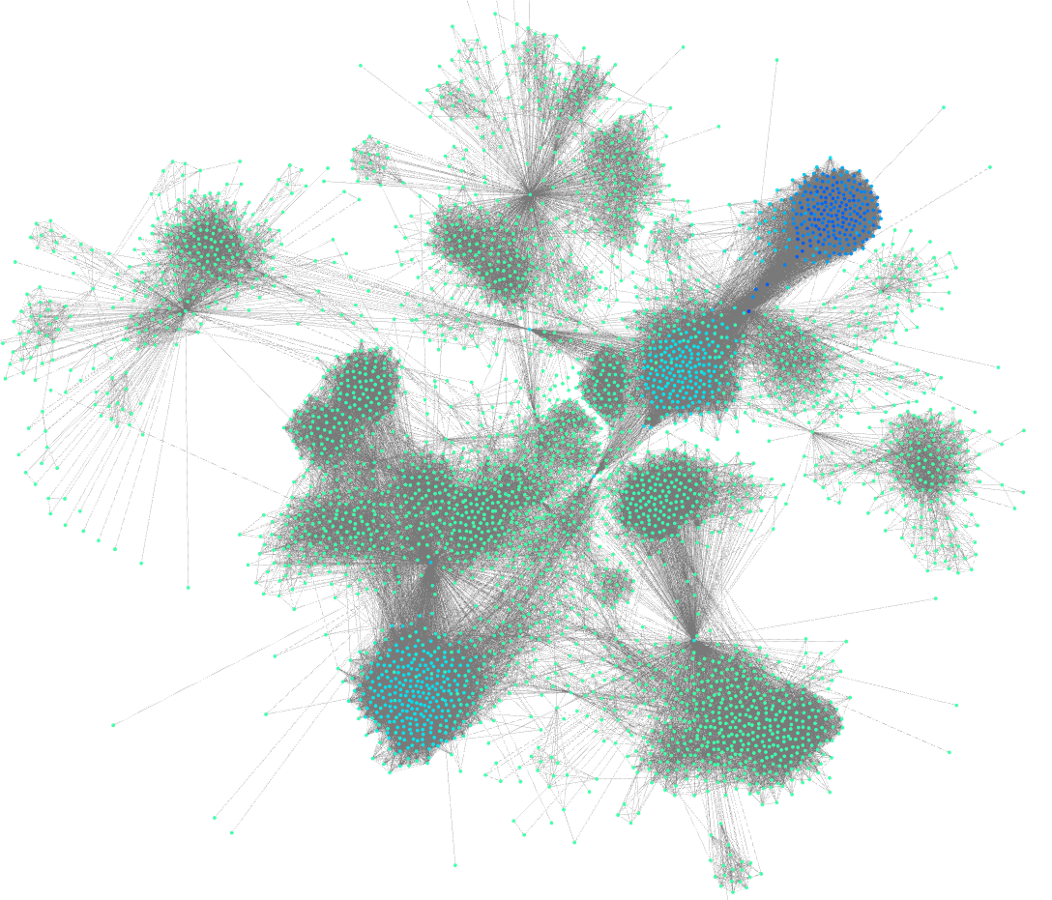
\includegraphics[width=0.5\textwidth]{img/facebook.png}
        \caption{Facebook Dataset Visualization}
    \end{figure}
    
    \subsection{\textbf{Computing Weight}}
    
    In this part, We applied preprocessing algorithm GRAMI on each graph to detect the set of metagraphs, and according to Metagraph-based Search, we only retained the symmetric ones. Then we train each edge's weight using part of Metagraph-based Search by replacing the original core formula with our improved TF-IDF-like weight formula, by this way we extracted all the features and obtained the corresponding scores, and the linear weighted summations are the edges' weights.
    
    \subsection{\textbf{Generating READS}}
    
    From the advanced READS algorithm above, the READS tree grows with the probabilities related to the linked edges' weights of the node, which are normalized beforehand. And the offline work only stored the next-list for each simulation, as known as $O(rn)$ space complexity.
    
    After this, online queries will returns results from One-to-all algorithm. And our experiment results are as following.
    
    \subsection{Results}
    
    We illustrate the average matching accuracy for LinkedIn and Facebook per query sample batch in Figure 4, where the size of each sample is 87 and 246, respectively. It's obvious that our algorithm has a better behavior on Facebook significantly, and the reason is also obvious. Facebook dataset has 10 types in total which includes details like work-project, while LinkedIn dataset only covers 4 rough types, that is to say Facebook dataset's sematic label has more tiny grain, and thus providing more credible evidence in the decision of weight scores.
    
    \begin{figure}[H]
        \centering
        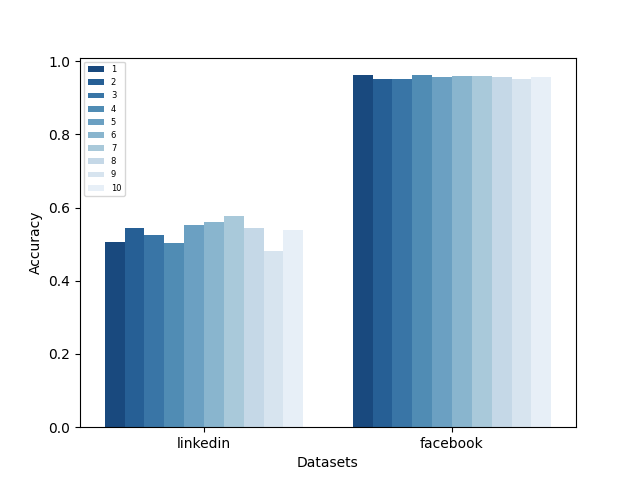
\includegraphics[width=0.5\textwidth]{img/linkedin-facebook.png}
        \caption{Query accuracy results for LinkedIn and Facebook}
    \end{figure}
    
    The first graph shows the similarity without semantic information for node 17, while the second shows the the similarity with semantic weight for the same node. As for the top 5 simrank nodes, original READS algorithm results to node 61,0,27,15 and 55, however, node 0 and node 27 both have nothing in common with node 17 at all in reality, actually they live in social circles without any intersection. On the other hand, our algorithm presents better results which are node 42,38,15,32 and 65, in which node 42 is truly considered as the most similar one with node 17 in our anticipation. On the contrary, the orighial READS gives 6,41,57,56 and 8 as top 5 dissimilar nodes for node 17, but unfortunately node 6 and node 57 are both like-minded friends with node 17. While our algorithm gives node 53,24,21,26 and 35, which are strangers with id 17 and totally different with node 17, reasonable. Though the man-made dataset may have some inevitable mistakes, generally our modified algorithm always shows a better ranking on similarity. 
    
    \begin{figure}[H]
        \centering
        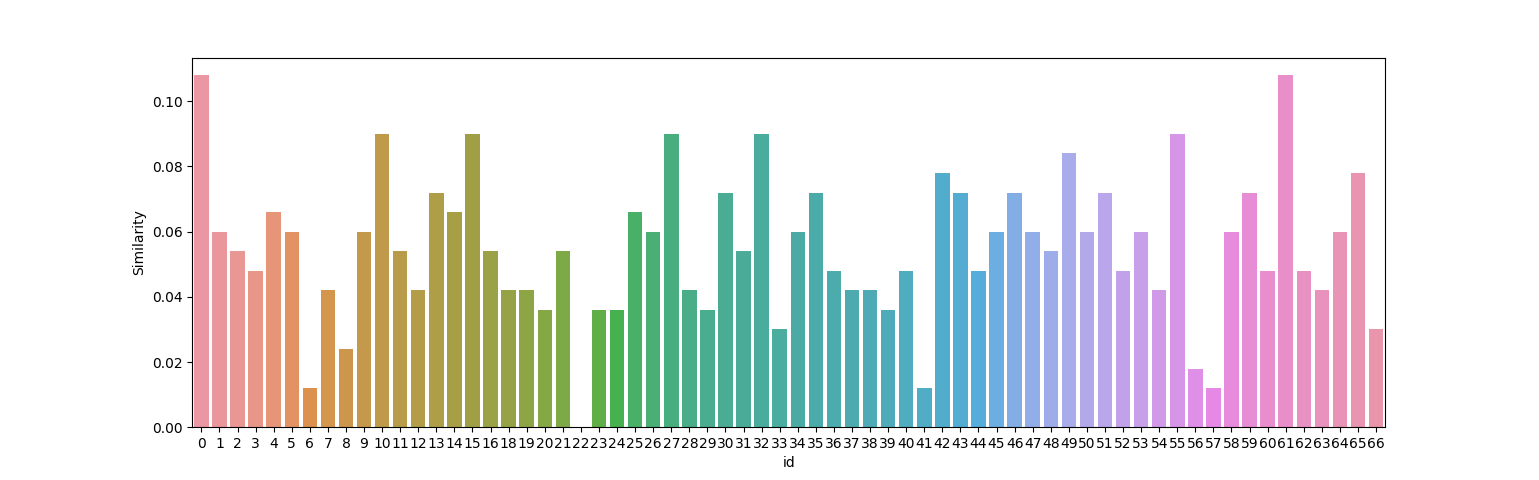
\includegraphics[width=\textwidth]{img/fudands-sample-1.png}
        \caption{FudanDS similarity sample (without semantic)}
    \end{figure}
    
    \begin{figure}[H]
        \centering
        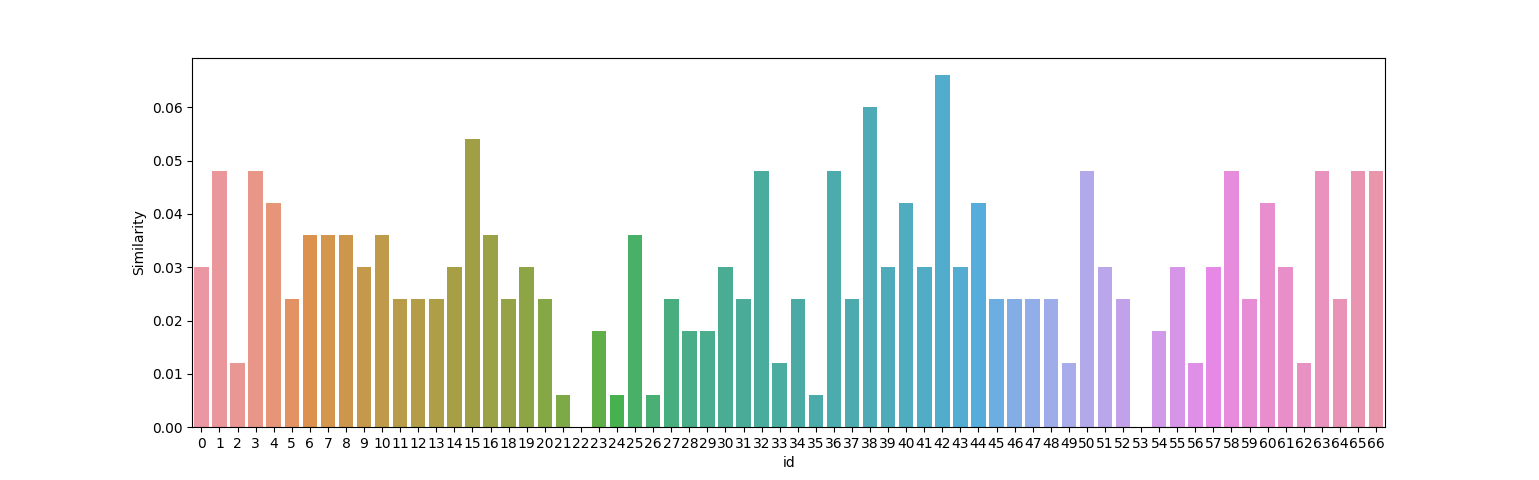
\includegraphics[width=\textwidth]{img/fudands-sample-2.png}
        \caption{FudanDS similarity sample (semantic)}
    \end{figure}


\bigskip

%------------------------------------------------

\section{Conclusion}
    
    To put it into a nutshell, MARS (Metagraph-based semAntic-boosting Reads Simrank) algorithm takes advantage of the semantic weighted information generated from metagraph and the linear space complexity inspired from READS. Furthermore, we improve the weighted calculation formula with the idea migrated from TF-IDF in LSA, which considers both semantic label's similarity and global semantic specificity.

\bigskip    

\begin{thebibliography}{99}
    \bibitem{ref1} Youngmann, B., Milo, T., Somech, A.: Boosting simrank with semantics. In: EDBT, pp. 37–48 (2019)
    \bibitem{ref2} Wang, X., Zhang, R., Lee, Y.-K., Sun, L., \& Moon, Y.-S. (Eds.). (2020). Web and Big Data. Lecture Notes in Computer Science. doi:10.1007/978-3-030-60259-8
    \bibitem{ref3} Fang, Y., Lin, W., Zheng, V. W., Wu, M., Chang, K. C.-C., \& Li, X.-L. (2016). Semantic proximity search on graphs with metagraph-based learning. 2016 IEEE 32nd International Conference on Data Engineering (ICDE). doi:10.1109/icde.2016.7498247
    \bibitem{ref4} Jiang, M., Fu, A. W.-C., \& Wong, R. C.-W. (2017). READS. Proceedings of the VLDB Endowment, 10(9), 937–948. doi:10.14778/3099622.3099625 
\end{thebibliography}
%----------------------------------------------------------------------------------------
%	REFERENCE LIST
%----------------------------------------------------------------------------------------

% \cite{Eureka}
% \printbibliography

%----------------------------------------------------------------------------------------

\end{document}
